\usepackage{fontspec}

\setsansfont{Palatino}[
    Path=./palatino/,
    Extension = .ttf,
    UprightFont=*-Roman,
    BoldFont=*-Bold,
    ItalicFont=*-Italic,
    BoldItalicFont=*-BoldItalic
]
\setmainfont{Palatino}

\usepackage[textwidth=0.86\paperwidth, textheight=0.86\paperheight]{geometry}
\usepackage{fancyhdr}
\usepackage{hyperref}
\usepackage{fontawesome5}
\usepackage{graphicx}
\usepackage{amssymb}
\usepackage{amsmath}

\newcommand{\R}{\mathbb{R}}

% \pagenumbering{gobble}
\pagestyle{fancy}
\fancyhead{} % clear all header fields
\fancyhead[R]{\href{https://hse24.fmin.xyz}{\faGem[regular]} \hspace{0.04cm} \href{https://github.com/MerkulovDaniil/hse24}{\faGithub} \hspace{0.07cm} \href{https://t.me/fminxyz}{\faTelegram}}
\fancyhead[L]{\href{https://fmin.xyz}{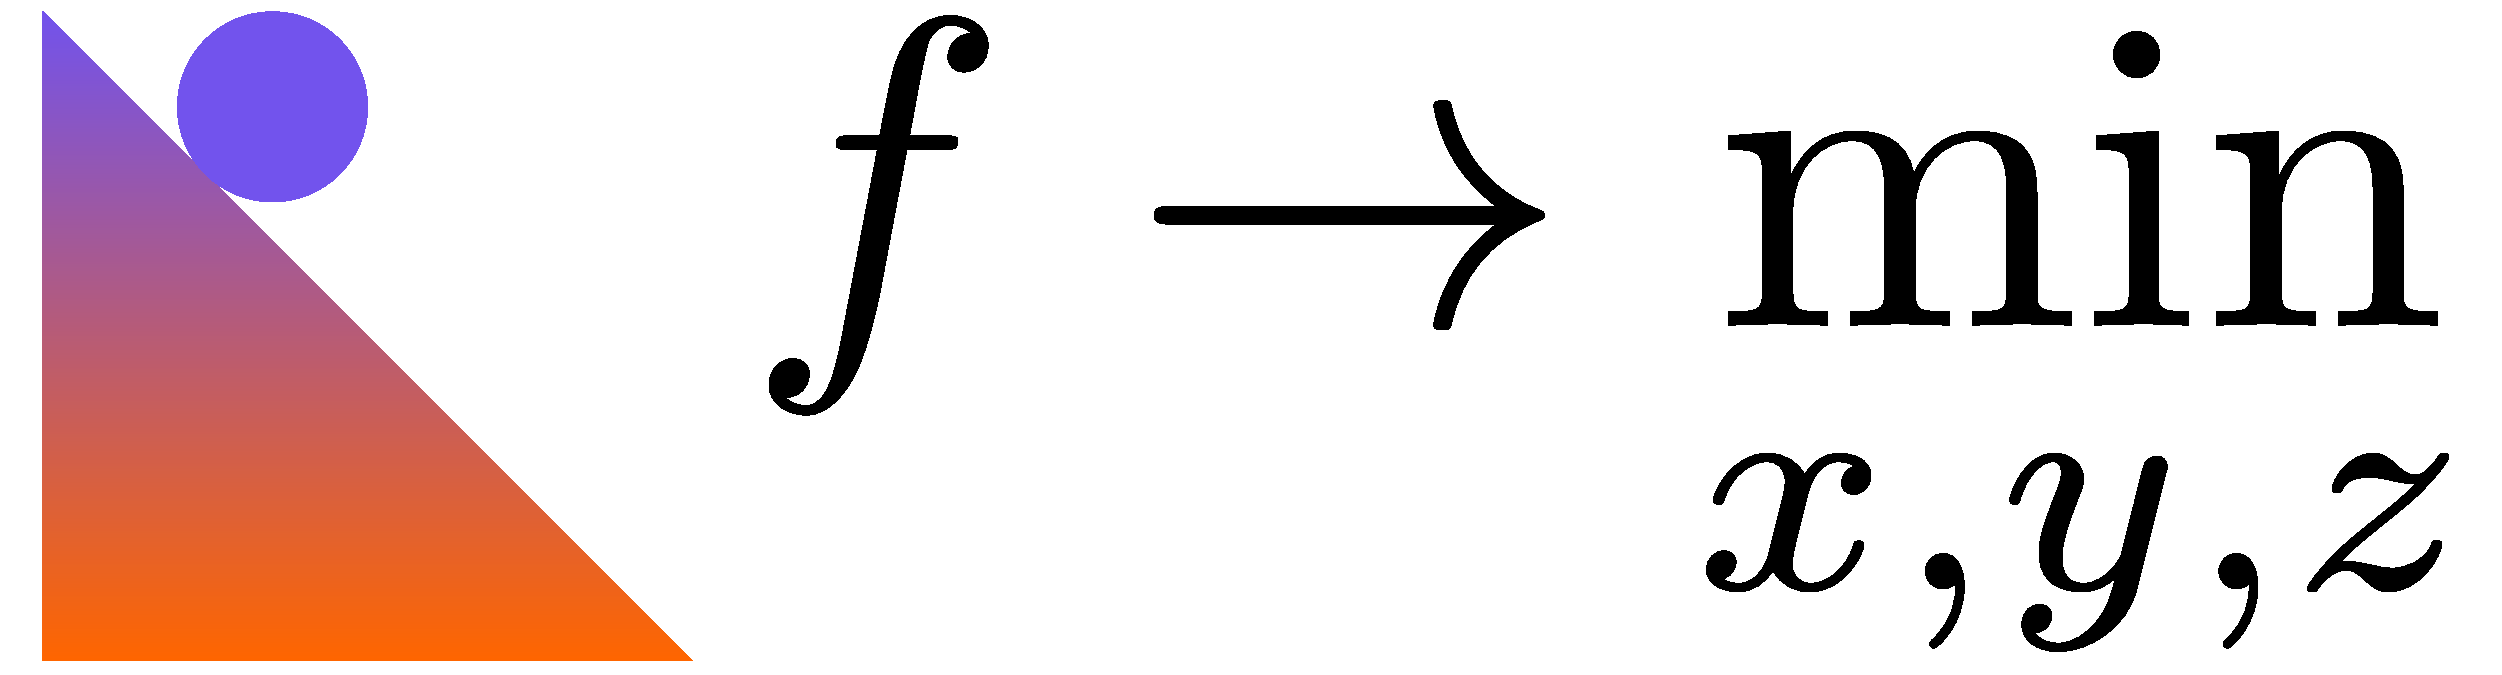
\includegraphics[height=0.35cm]{logo.pdf}} \hspace{2pt} \textbf{Методы оптимизации в машинном обучении. ФКН ВШЭ. 2024}}